\documentclass{article}
\usepackage[submission]{colm2026_conference}

\usepackage{microtype}
\usepackage{hyperref}
\usepackage{url}
\usepackage{booktabs}
\usepackage{amsmath,amssymb}
\usepackage{graphicx}
\usepackage{xcolor}
\usepackage{enumitem}
\usepackage{subcaption}
\newcommand{\nicefrac}[2]{#1/#2}
\usepackage{caption}
\usepackage{pifont}
\usepackage{lineno}

\definecolor{darkblue}{rgb}{0, 0, 0.5}
\hypersetup{colorlinks=true, citecolor=darkblue, linkcolor=darkblue, urlcolor=darkblue}

\captionsetup{font=small, labelfont=bf}

\title{SenseMath: A Controlled Benchmark for Shortcut-Sensitive Numerical Reasoning in Large Language Models}

\author{
  Anonymous Submission
}

\begin{document}

\ifcolmsubmission
\linenumbers
\fi

\maketitle

\begin{abstract}
Large language models default to step-by-step computation even when efficient numerical shortcuts exist, yet no benchmark isolates whether this reflects a strategic deficit or merely a prompting one.
We introduce \textsc{SenseMath}, a controlled benchmark that measures prompt-sensitive shortcut exploitation on matched item families.
The benchmark comprises 1{,}600 families spanning 8 categories (6 core number-sense types plus equation reasoning and option elimination) and 4 digit scales ($d \in \{2, 4, 8, 16\}$), each instantiated in strong-shortcut, weak-shortcut, and control variants that share identical surface complexity but differ in shortcut availability.
We evaluate 5 models (GPT-4o-mini, GPT-4.1-mini, Qwen3-30B, Qwen3-8B, and Llama-3.1-8B) under chain-of-thought (CoT), number-sense (NC), and strict prompting conditions (72{,}000 total inferences).
We find an asymmetric prompting effect: NS prompting maintains or improves accuracy on shortcut-amenable items while selectively reducing accuracy on matched controls, with the pattern most pronounced at $d{=}4$.
Per-category radar profiles reveal that models show selective strengths and reversals across shortcut types: Qwen models excel on magnitude estimation and structural shortcuts, while GPT-4o-mini leads on cancellation, equation reasoning, and option elimination.
A three-level evaluation framework (Use, Judge, Generate) confirms that shortcut exploitation, shortcut recognition, and shortcut construction dissociate across models.

\end{abstract}

\section{Introduction}
\label{sec:introduction}

Consider $98 \times 14$.
A skilled human reasoner recognises this as $(100 - 2) \times 14 = 1{,}400 - 28 = 1{,}372$, a structural shortcut that sidesteps column multiplication entirely.
When the operand shifts to $73 \times 14$, no comparable decomposition presents itself and the same reasoner reverts to standard arithmetic.
The ability to detect and exploit such structural opportunities, rather than applying a uniform procedure to every problem, is the hallmark of \emph{number sense} \citep{mcintosh1992proposed, reys1991number}.

Large language models, by contrast, tend to default to verbose chain-of-thought computation regardless of whether a problem admits a shortcut \citep{wei2022chain, kojima2022large}.
This raises a basic question: do LLMs possess latent shortcut-sensitive reasoning that can be selectively activated, or do they lack this capacity entirely?
The question has been difficult to answer because existing benchmarks are not designed to test it.
GSM8K \citep{cobbe2021gsm8k} and MATH \citep{hendrycks2021math} measure whether a model reaches the correct answer, not whether it selects an efficient strategy to get there.
A model that applies long multiplication to every problem and a model that recognises algebraic shortcuts receive identical scores, provided both arrive at the right answer.
Strategy selection, the core of number sense, is invisible to accuracy-only evaluation.

We argue that measuring number sense requires a different experimental design: one that holds problem structure constant while varying shortcut availability, then tests whether prompting interventions produce differential effects across matched item variants.
This logic parallels factorial designs in cognitive psychology, where the interaction between task condition and experimental manipulation is the quantity of interest, not main effects alone.

\paragraph{Research questions.}
We address three questions:
\begin{enumerate}[leftmargin=*,itemsep=2pt]
    \item \textbf{Selective activation.} Does number-sense prompting improve accuracy on shortcut-amenable items more than on matched controls?
    \item \textbf{Cross-model variation.} Do different models show qualitatively different shortcut profiles across categories, rather than uniformly scaling with model size?
    \item \textbf{Multi-dimensional structure.} Is number sense a single axis or a collection of dissociable competencies (e.g., magnitude estimation vs.\ cancellation vs.\ structural decomposition)?
\end{enumerate}

\paragraph{The \textsc{SenseMath} benchmark.}
To answer these questions, we introduce \textsc{SenseMath}, a controlled benchmark of 1{,}600 item families spanning 8 categories and 4 digit scales ($d \in \{2, 4, 8, 16\}$).
Six \emph{core} categories target established number-sense competencies (magnitude estimation, structural shortcuts, relative distance, cancellation, compatible numbers, landmark comparison); two \emph{extension} categories probe reasoning-level and option-level shortcuts (equation reasoning and option elimination, respectively).
Each family contains three variants (strong-shortcut, weak-shortcut, and control) that share the same template and digit scale but differ in whether a clean shortcut is available.
All items use a four-option multiple-choice format with answers extracted via \boxed{} to ensure unambiguous scoring.
An overview of the benchmark design appears in Figure~\ref{fig:overview}.

\paragraph{Key findings.}
We evaluate five models (GPT-4o-mini, GPT-4.1-mini, Qwen3-30B, Qwen3-8B, and Llama-3.1-8B) under chain-of-thought (CoT), number-sense (NC), and strict prompting conditions, totalling 72{,}000 inferences.
We find that a category-agnostic NS prompt, which mentions only ``easy calculations'' and ``mathematical intuition'' without naming any specific shortcut, produces an asymmetric effect: accuracy on shortcut-amenable items is maintained or improved while accuracy on matched controls drops, most consistently at $d{=}4$.
The per-category bar charts (Figure~\ref{fig:bar_d4}) reveal that models show selective strengths and reversals across shortcut types: Qwen models lead on magnitude estimation and structural shortcuts, while GPT-4o-mini dominates cancellation, equation reasoning, and option elimination.
No single model uniformly outperforms the others, suggesting that number sense is not a monolithic capability but a collection of partially independent dimensions.

\paragraph{Contributions.}
We make four contributions:
\begin{enumerate}[leftmargin=*,itemsep=2pt]
    \item A controlled benchmark (\textsc{SenseMath}) with 1{,}600 matched families across 8 categories and 4 scales, enabling factorial analysis of shortcut exploitation under prompt manipulation.
    \item Evidence that a category-agnostic NS prompt induces a broad shortcut-seeking mode: accuracy on shortcut-amenable items is maintained or improved while control accuracy drops. The effect is statistically reliable for two of five models (GPT-4o-mini, Qwen3-8B), with the same directional pattern in two others.
    \item A three-level evaluation framework spanning Use (solve), Judge (recognise), and Generate (create), revealing crossed dissociations in shortcut competence across models.
    \item Per-category radar analysis showing that different models excel at different shortcut types, establishing number sense as a multi-dimensional construct rather than a single ability.
\end{enumerate}

\begin{figure}[t]
    \centering
    
\includegraphics[width=0.95\textwidth]{figures/fig1_overview.pdf}
    \caption{\textsc{SenseMath} overview. Each item family consists of matched strong-shortcut, weak-shortcut, and control variants administered under CoT and NS prompting. The matched design isolates selective shortcut exploitation from general prompt effects.}
    \label{fig:overview}
\end{figure}

% ── 2. Related Work ───────────────────────────────────────────────────────────
\section{Related Work}
\label{sec:related}

\paragraph{Mathematical reasoning benchmarks.}
The dominant paradigm for evaluating mathematical ability in LLMs relies on end-to-end accuracy.
GSM8K \citep{cobbe2021training} tests grade-school word problems; MATH \citep{hendrycks2021measuring} covers competition-level algebra, geometry, and number theory; MathBench \citep{liu2024mathbench} provides multi-level curricula; MathVista \citep{lu2024mathvista} extends evaluation to visual contexts; and selected BIG-Bench tasks \citep{srivastava2023beyond} probe arithmetic and logical reasoning.
Recent diagnostic work has exposed fragilities behind high aggregate scores: GSM-Symbolic \citep{mirzadeh2024gsmsymbolic} shows that adding a single irrelevant clause can drop accuracy by up to 65\%, and MATH-Perturb \citep{huang2025mathperturb} demonstrates that structural perturbations defeat memorised solution paths.
Chain-of-thought prompting \citep{wei2022chain} and its variants \citep{wang2023selfconsistency,yao2023tree} have substantially raised scores on all of these benchmarks.
However, the shared limitation is that they treat every correct answer identically regardless of the reasoning path that produced it.
A model that cross-multiplies two fractions and a model that recognises both are near $\nicefrac{1}{2}$ receive the same credit.
This conflation obscures whether LLMs possess efficient, flexible numerical reasoning or merely execute brute-force procedures.
\textsc{SenseMath} addresses this gap by controlling the \emph{availability} of shortcut strategies across matched item variants, so that accuracy differences are attributable to strategy selection rather than problem difficulty.

\paragraph{Efficient and compressed reasoning.}
A growing line of work aims to preserve reasoning quality while reducing token expenditure.
Chain of Draft \citep{kim2024chain} generates minimal intermediate steps instead of verbose chains.
Sketch-of-Thought \citep{aytes2025sketch} uses cognitive-inspired paradigms to reduce token use by up to 84\%.
Token-Budget-Aware reasoning \citep{han2024tokenbudget} inserts explicit budgets into prompts, compressing verbose reasoning by 67\% with no accuracy loss.
\citet{chen2024overthinking} show that O1-like models waste computation on trivial problems, precisely the failure mode that number-sense shortcuts are designed to avoid.
These approaches share a common assumption: the underlying \emph{strategy} is fixed (typically step-by-step computation), and the goal is to express it more concisely.
By contrast, number sense involves switching to a qualitatively different strategy (estimation, benchmarking, or structural decomposition) that is inherently shorter because it skips unnecessary computation.
Our work is therefore orthogonal: efficient-reasoning methods compress the \emph{same} strategy; \textsc{SenseMath} measures whether models can \emph{select a different} strategy.

\paragraph{Number sense in mathematics education.}
The concept of number sense originates in the mathematics education literature.
\citet{mcintosh1992proposed} define it as ``a person's general understanding of number and operations along with the ability and inclination to use this understanding in flexible ways to make mathematical judgements.''
\citet{reys1991number} identify key components including magnitude estimation, use of benchmarks (e.g., $\nicefrac{1}{2}$, powers of 10), and recognition of numerical structure (e.g., near-cancellation, compatible-number pairs).
\citet{sowder1992making} emphasise that number sense is not a single skill but a disposition to choose efficient paths. We would now call this a \emph{meta-cognitive strategy selection} ability.
\citet{yang2003assessing} operationalise these ideas into validated test instruments for school-age children.
Crucially, this literature demonstrates that expert human reasoners do not uniformly apply algorithmic procedures; they adaptively select shortcuts when the problem structure permits.
We adopt this taxonomy as the category system for \textsc{SenseMath}.

\paragraph{Numerical cognition in LLMs.}
Recent work has begun probing whether LLMs possess numerical understanding beyond surface-level pattern matching.
\citet{rahman2025fragile} test LLMs on escalating numerical tasks and find strong deterministic performance but failure on heuristic-search problems, suggesting a ``fragile number sense.''
\citet{li2025numeracy} introduce NumericBench covering six numeracy capabilities and expose systematic gaps in basic numerical skills.
At the mechanistic level, \citet{nikankin2024arithmetic} show that LLMs solve arithmetic using sparse neuron-level heuristics rather than learned algorithms, providing a circuit-level explanation for why models may or may not exploit human-like shortcuts.
\citet{yan2025grasp} find that models achieve high numeric accuracy on addition but violate commutativity in up to 20\% of cases, directly relevant to our equation-reasoning category.
\textsc{SenseMath} complements these investigations by testing whether shortcut-sensitive reasoning can be \emph{selectively activated} through prompting, rather than probing for its unconditional presence.

\paragraph{Diagnostic and contrastive evaluation.}
Standard accuracy-based benchmarks can be ``gamed'' by surface-level cues.
Contrast sets \citep{gardner2020evaluating} address this by perturbing evaluation examples to create minimally different instances that change the gold label, exposing model brittleness.
CheckList \citep{ribeiro2020beyond} provides a task-agnostic framework of behavioural tests (invariance, directional expectation, and minimum functionality) applied to NLP models.
BIG-Bench Hard \citep{suzgun2023challenging} isolates a subset of BIG-Bench tasks where LLMs initially fail, enabling targeted analysis of failure modes.
These works share the philosophy that controlled variation is more informative than aggregate accuracy.
\textsc{SenseMath} extends this philosophy to mathematical reasoning: rather than perturbing surface text, we perturb the \emph{numerical structure} of problems to toggle shortcut availability while holding surface complexity constant.
The family-matching design (strong-shortcut, weak-shortcut, and control variants sharing the same template and digit scale) directly parallels the contrast-set methodology, but targets strategy selection rather than label robustness.

\paragraph{Positioning of \textsc{SenseMath}.}
To our knowledge, \textsc{SenseMath} is the first benchmark that \emph{controls shortcut availability at the item level} within matched families.
Existing math benchmarks vary difficulty but not strategy affordance; existing contrastive benchmarks perturb text but not numerical structure; existing efficiency work compresses a fixed strategy rather than evaluating strategy choice.
\textsc{SenseMath} occupies the intersection: each item family holds surface complexity fixed while toggling whether a number-sense shortcut is viable, enabling causal attribution of performance differences to strategy selection.
The family-matching design further supports within-family statistical tests (permutation-based asymmetry tests) that are impossible with unpaired item sets.

% ── 3. SenseMath Benchmark ────────────────────────────────────────────────────
\section{The \textsc{SenseMath} Benchmark}
\label{sec:benchmark}

\textsc{SenseMath} is a controlled benchmark for measuring whether LLMs can exploit number-sense shortcuts. This section describes our design philosophy, category taxonomy, programmatic generation pipeline, and evaluation framework.

\subsection{Design Philosophy}
\label{sec:design}

The central question is whether LLMs can reduce computation when a problem's numerical structure permits it. We operationalise this through three design choices.

\textbf{Shortcut definition.}
A shortcut is \emph{effective} if it reduces the problem to operations trivially executable in one's head: single-digit arithmetic, multiplication by powers of 10, or simple addition after simplification.
A shortcut is \emph{not} effective if the simplified form still requires multi-digit multiplication (e.g., rounding $5{,}374 \times 2{,}169$ to $5{,}400 \times 2{,}200$ does not meaningfully reduce computation), or if the approximation cannot uniquely identify the correct answer among the given options.

\textbf{Matched family design.}
Each item belongs to a \emph{family} containing three variants: \emph{strong} (clean shortcut available), \emph{weak} (partial shortcut requiring more effort), and \emph{control} (no effective shortcut). All three share the same template and digit scale, differing only in numerical values. This matched design lets us attribute accuracy differences to shortcut availability rather than problem difficulty.

\textbf{Three-level evaluation.}
We evaluate number sense at three levels of cognitive demand:
\emph{Use} (can the model solve the problem more accurately when encouraged to use shortcuts?),
\emph{Judge} (can the model recognise when a shortcut applies or identify a shortcut strategy in a solution?), and
\emph{Generate} (can the model construct new shortcut/control problem pairs?).

\subsection{Categories}
\label{sec:categories}

\textsc{SenseMath} spans 8 categories organised into three tiers based on where the shortcut operates.

\textbf{Tier 1: Problem-level shortcuts} target competencies from the mathematics education literature \citep{mcintosh1992proposed,reys1991number}.
\emph{Magnitude estimation (ME)}: rounding operands to nearby powers of 10.
\emph{Structural shortcuts (SS)}: exploiting algebraic identities near round numbers (e.g., $99 \times 37 = (100{-}1) \times 37$).
\emph{Relative distance (RD)}: comparing fractions by their distance from a benchmark (e.g., $\nicefrac{1}{2}$).
\emph{Cancellation (CI)}: near-cancellation in $A + B - C$ when $B \approx C$.
\emph{Compatible numbers (CN)}: rounding to product-friendly pairs (e.g., $250 \times 4000$).
\emph{Landmark comparison (LC)}: comparing percentages to landmarks (e.g., $49\% \approx 50\%$).

\textbf{Tier 2: Reasoning-level shortcut.}
\emph{Equation reasoning (ER)}: recognising algebraic identities (commutativity, common-term cancellation) in fill-in-the-blank equations, reducing multi-step algebra to a single observation.

\textbf{Tier 3: Option-level shortcut.}
\emph{Option elimination (OE)}: ruling out answer choices by quick feasibility checks (trailing digit, parity, magnitude) without computing the exact answer.

Example items for each category are provided in Appendix~\ref{sec:appendix_examples}.

\subsection{Program-Based Generation}
\label{sec:generation}

All items are generated programmatically via category-specific Python generators with rejection sampling. This ensures:
(i) 100\% answer correctness by construction (exact arithmetic at generation time);
(ii) distractors that share the last 50\% of digits with the correct answer (arithmetic categories) or fall within $\pm 0.1$ decimal (fraction categories), preventing option-level elimination;
(iii) strong and control variants within a family that differ only in numerical values, not template structure;
(iv) operands in control items that are ``hard numbers'' (last two digits in [25, 75], not divisible by 10, not near round boundaries), verified by automated checks.

The benchmark spans 4 digit scales ($d \in \{2, 4, 8, 16\}$), yielding $8 \text{ categories} \times 50 \text{ families} \times 4 \text{ scales} = 1{,}600$ families and $4{,}800$ individual items.
Scaling operand size increases computational load while leaving shortcut applicability unchanged in strong variants.

\subsection{Prompting Conditions}
\label{sec:conditions}

Each item is administered under three prompting conditions that differ in how strongly they encourage or suppress shortcut strategies:

\textbf{CoT} (chain-of-thought): standard step-by-step reasoning instruction.

\textbf{NS} (number-sense): encourages mathematical intuition and easy calculations. Crucially, the NS prompt does \emph{not} name any specific shortcut type; it is deliberately category-agnostic.

\textbf{Strict}: explicitly forbids shortcuts, requiring digit-by-digit computation. Serves as a negative control.

All conditions require answers inside \texttt{\textbackslash boxed\{\}} for unambiguous extraction. Full prompt templates are provided in Appendix~\ref{sec:appendix_prompts}.

\subsection{Evaluation Metrics}
\label{sec:metrics}

\textbf{Accuracy.} The primary metric is per-variant accuracy under each prompting condition. The key signature of number-sense exploitation is an asymmetric prompting effect: NS prompting maintains or improves accuracy on strong items while reducing accuracy on control items.

\textbf{NS rate.} To directly measure strategy choice beyond accuracy, we use GPT-4.1-mini as an automated judge to classify each model response as SHORTCUT or COMPUTATION. This provides a process-level measure of whether NS prompting actually changes the reasoning strategy, not just the final answer.

\textbf{Normalised improvement.} To compare across categories with different CoT baselines, we report the normalised improvement $(\text{NS} - \text{CoT}) / (1 - \text{CoT})$, which measures what fraction of the remaining accuracy gap NS captures. A value of $+1$ means NS closes the entire remaining gap; $0$ means no change; negative means NS hurts performance.

\subsection{Judge and Generate Tasks}
\label{sec:judge_gen}

Beyond Use-level accuracy, we evaluate declarative and constructive shortcut competence.

\textbf{Judge tasks.} J1 presents a problem with options and asks whether it could be solved faster with mental math (YES/NO). J2 presents a problem with a solution and asks whether the solution used a shortcut or computation strategy (SHORTCUT/COMPUTATION). These measure whether models can \emph{recognise} shortcut applicability (J1) and \emph{identify} strategy type (J2).

\textbf{Generate task (G2).} Given a category description and one example, models generate a new strong/control problem pair. Generated items are verified by 6 deterministic code checks (answer correctness, shortcut existence, control blocks shortcut, family matching, novelty, digit scale). This measures whether models can \emph{construct} shortcut-amenable problems.

Full task specifications and verification details are provided in Appendix~\ref{sec:appendix_tasks}.

\section{Experiments}
\label{sec:experiments}

This section presents the empirical evaluation of \textsc{SenseMath}.
We describe the experimental setup (\S\ref{sec:exp_setup}), report the main prompting asymmetry (\S\ref{sec:main_result}), per-category analysis (\S\ref{sec:per_category}), strict-prompt validation (\S\ref{sec:strict}), and CoT strategy analysis (\S\ref{sec:cot_strategy}).

% ─────────────────────────────────────────────────────────────────────────────
\subsection{Experimental Setup}
\label{sec:exp_setup}

\paragraph{Models.}
We evaluate five instruction-tuned models spanning three families:
Qwen3-30B and Qwen3-8B \citep{qwen2025qwen3},
Llama-3.1-8B-Instruct \citep{grattafiori2024llama},
and GPT-4o-mini and GPT-4.1-mini \citep{openai2024gpt4o}.
GPT-4.1-mini is a more capable successor to GPT-4o-mini that achieves near-ceiling CoT accuracy on \textsc{SenseMath} at $d{=}4$, providing an important reference point for how strong baseline performance constrains the prompting asymmetry.
Open-weight models are served via vLLM with tensor parallelism; GPT models are accessed through the OpenAI API.
All inferences use greedy decoding (temperature$\,{=}\,0$) and $\texttt{max\_tokens}{=}512$.

\paragraph{Conditions.}
Each of the 1{,}600 item families is evaluated under three prompting conditions (CoT, NS, Strict) across three variants (strong, weak, control), yielding $1{,}600 \times 3 \times 3 = 14{,}400$ inferences per model and \textbf{72{,}000 total inferences} across five models.

\paragraph{Metrics.}
Our primary analysis compares accuracy on strong-shortcut versus control items under NS and CoT prompting, supplemented by the NS rate (shortcut strategy classification by GPT-4.1-mini judge) and the normalised improvement metric defined in \S\ref{sec:metrics}.

% ─────────────────────────────────────────────────────────────────────────────
\subsection{Main Result: Prompting Asymmetry at $d{=}4$}
\label{sec:main_result}

Table~\ref{tab:main_results} presents per-condition accuracies on strong-shortcut and control items across all four digit scales for five models.

\begin{table*}[t]
  \centering
  \small
  \setlength{\tabcolsep}{2.5pt}
  \caption{Per-condition results across digit scales for five models. Acc = accuracy; NS\% = shortcut-strategy rate classified by GPT-4.1-mini judge. $S$ = strong-shortcut variant, $W$ = weak-shortcut variant, $C$ = control variant. All numbers are percentages (rounded to integers).}
  \label{tab:main_results}
  \begin{tabular}{ll|rrr|rrr|rrr|rrr}
    \toprule
    \textbf{Model} & \textbf{Metric} & \multicolumn{3}{c|}{$d=2$ (\%)} & \multicolumn{3}{c|}{$d=4$ (\%)} & \multicolumn{3}{c|}{$d=8$ (\%)} & \multicolumn{3}{c}{$d=16$ (\%)} \\
     &  & $S$ & $W$ & $C$ & $S$ & $W$ & $C$ & $S$ & $W$ & $C$ & $S$ & $W$ & $C$ \\
    \midrule
    GPT-4o-mini & $\text{Acc}_{\text{CoT}}$ & 88 & 88 & 85 & 78 & 70 & 65 & 75 & 62 & 55 & 67 & 53 & 46 \\
     & $\text{Acc}_{\text{NS}}$ & 92 & 92 & 87 & 84 & 72 & 63 & 82 & 73 & 62 & 70 & 59 & 51 \\
     & $\text{NS\%}_{\text{CoT}}$ & 28 & 18 & 24 & 27 & 16 & 18 & 36 & 21 & 22 & 37 & 27 & 22 \\
     & $\text{NS\%}_{\text{NS}}$ & 46 & 37 & 44 & 77 & 65 & 78 & 84 & 76 & 80 & 90 & 80 & 90 \\
    \midrule
    GPT-4.1-mini & $\text{Acc}_{\text{CoT}}$ & 99 & 99 & 99 & 88 & 89 & 76 & 80 & 72 & 65 & 74 & 58 & 60 \\
     & $\text{Acc}_{\text{NS}}$ & 100 & 100 & 100 & 96 & 94 & 83 & 95 & 86 & 83 & 86 & 70 & 69 \\
     & $\text{NS\%}_{\text{CoT}}$ & 16 & 7 & 7 & 20 & 4 & 1 & 46 & 22 & 37 & 57 & 34 & 48 \\
     & $\text{NS\%}_{\text{NS}}$ & 70 & 58 & 62 & 68 & 50 & 70 & 80 & 66 & 78 & 87 & 86 & 87 \\
    \midrule
    Qwen3-8B & $\text{Acc}_{\text{CoT}}$ & 97 & 99 & 98 & 74 & 70 & 65 & 70 & 62 & 59 & 56 & 48 & 50 \\
     & $\text{Acc}_{\text{NS}}$ & 98 & 98 & 95 & 72 & 55 & 53 & 70 & 55 & 52 & 56 & 38 & 34 \\
     & $\text{NS\%}_{\text{CoT}}$ & 30 & 17 & 14 & 37 & 16 & 25 & 55 & 26 & 44 & 56 & 36 & 46 \\
     & $\text{NS\%}_{\text{NS}}$ & 66 & 56 & 55 & 86 & 72 & 88 & 87 & 79 & 90 & 90 & 88 & 98 \\
    \midrule
    Qwen3-30B-A3B & $\text{Acc}_{\text{CoT}}$ & 100 & 100 & 98 & 68 & 58 & 56 & 57 & 44 & 47 & 48 & 30 & 31 \\
     & $\text{Acc}_{\text{NS}}$ & 100 & 100 & 100 & 73 & 68 & 56 & 74 & 50 & 52 & 60 & 42 & 44 \\
     & $\text{NS\%}_{\text{CoT}}$ & 26 & 15 & 15 & 39 & 22 & 33 & 60 & 39 & 47 & 59 & 42 & 52 \\
     & $\text{NS\%}_{\text{NS}}$ & 86 & 77 & 76 & 86 & 84 & 92 & 89 & 84 & 83 & 94 & 96 & 98 \\
    \midrule
    Llama-3.1-8B & $\text{Acc}_{\text{CoT}}$ & 82 & 76 & 80 & 66 & 70 & 58 & 62 & 53 & 51 & 51 & 36 & 33 \\
     & $\text{Acc}_{\text{NS}}$ & 74 & 70 & 68 & 59 & 56 & 55 & 57 & 48 & 50 & 55 & 45 & 42 \\
     & $\text{NS\%}_{\text{CoT}}$ & 26 & 24 & 25 & 31 & 25 & 24 & 37 & 24 & 24 & 40 & 33 & 26 \\
     & $\text{NS\%}_{\text{NS}}$ & 62 & 58 & 59 & 78 & 76 & 69 & 86 & 82 & 90 & 92 & 87 & 86 \\
    \bottomrule
  \end{tabular}
\end{table*}


The key pattern across models is an asymmetric response to NS prompting: on strong-shortcut items, NS either maintains or slightly improves accuracy relative to CoT, whereas on control items NS consistently reduces accuracy.
For GPT-4o-mini at $d{=}4$, NS raises strong-shortcut accuracy to 84.5\% (vs.\ 78.2\% under CoT) while control accuracy drops from 64.8\% to 63.0\%.
Qwen3-8B shows a more nuanced pattern: strong accuracy holds steady (74.2\%$\to$72.0\%) while control drops (65.0\%$\to$53.2\%).
GPT-4.1-mini shows a large NS improvement on strong items (87.8\%$\to$96.5\%) while control also improves but less so (76.5\%$\to$83.2\%), reflecting near-ceiling capacity.
Qwen3-30B shows NS improving both strong and control, but with a larger boost on strong items (68.0\%$\to$72.8\% vs.\ 55.5\%$\to$56.5\%).
Llama-3.1-8B is the exception: NS degrades accuracy on strong items (66.5\%$\to$59.0\%) while control changes minimally (57.8\%$\to$54.8\%).

Bootstrap 95\% confidence intervals (10,000 resamples) for the strong-vs-control accuracy differential confirm that the asymmetry is reliable for GPT-4o-mini (+0.080 [+0.015, +0.147]) and Qwen3-8B (+0.095 [+0.032, +0.158]), while GPT-4.1-mini (+0.020 [$-$0.035, +0.075]), Qwen3-30B (+0.037 [$-$0.020, +0.095]), and Llama-3.1-8B ($-$0.045 [$-$0.125, +0.035]) include zero.

\paragraph{Dose-response pattern.}
The weak-shortcut variant provides an intermediate condition between strong and control.
At $d{=}4$ under NS, all five models show accuracy ordered as \{strong, weak\} $>$ control: GPT-4o-mini (84.5\%, 71.8\%, 63.0\%), GPT-4.1-mini (96.5\%, 94.0\%, 83.2\%), Qwen3-8B (72.0\%, 54.8\%, 53.2\%), Qwen3-30B (72.8\%, 68.5\%, 56.5\%), and Llama-3.1-8B (59.0\%, 56.0\%, 54.8\%).
In all cases, the gap between shortcut-bearing variants (strong and weak) and the control variant is substantially larger than the gap between strong and weak themselves.
This pattern is consistent with the mechanism identified by the strategy-use analysis: NS induces shortcut attempts on all items, and accuracy reflects whether a viable shortcut exists (strong and weak) or not (control).

\begin{figure*}[t]
\centering
\small
\fbox{\parbox{0.96\textwidth}{%
\textbf{Case 1: magnitude\_estimation} (Qwen3-8B, $d{=}4$) \hfill \textit{Answer: (A) 103{,}020{,}000}\\
\textit{Which is the best estimate for $10100 \times 10200$?} \quad (A) 103020000 \quad (B) 103020010 \quad (C) 103020020 \quad (D) 103019990\\[4pt]
%
\textbf{CoT response} (wrong, picks C):\\
{\footnotesize\ttfamily
We are asked to estimate the value of: $10^{100} \times 10^{200}$\\
Step 1: Use the properties of exponents. $10^a \times 10^b = 10^{a + b}$. So: $10^{100} \times 10^{200} = 10^{300}$\\
Step 2: Compare with the answer choices: (A) $10^{3020000}$ (B) $10^{3020010}$ (C) $10^{3020020}$ (D) $10^{3019990}$\\
Wait --- this is not the same as $10^{300}$! These choices are way too large. There's a misinterpretation\ldots\\
\mbox{}\hfill[\textit{continues for 1{,}275 tokens, eventually picks C}]}\\[4pt]
%
\textbf{NS response} (correct, picks A):\\
{\footnotesize\ttfamily
We are asked to estimate: $10100 \times 10200$\\
Step 1: Both numbers are close to 10{,}000. Write as: $10100 = 10000 + 100$, $10200 = 10000 + 200$\\
$(10000 + 100)(10000 + 200) = 10000^2 + 10000 \times 300 + 100 \times 200 = 100{,}000{,}000 + 3{,}000{,}000 + 20{,}000 = 103{,}020{,}000$\\
\mbox{}\hfill$\boxed{A}$}\\[4pt]
\textit{Analysis:} CoT misparses ``10100'' as $10^{100}$ (an exponent), leading to 1{,}275 tokens of confused reasoning. NS reads the integers correctly and applies FOIL decomposition in 3 steps.
}}
\caption{Case study: CoT fails but NS succeeds (Qwen3-8B, magnitude\_estimation, strong-shortcut, $d{=}4$). Actual model output shown verbatim. CoT misparses integers as exponents; NS decomposes correctly.}
\label{fig:case_study}
\end{figure*}

The $d{=}4$ scale appears to occupy a ``sweet spot'' where problems are difficult enough that CoT computation is error-prone, yet the digit scale is small enough that shortcut strategies remain executable.
At $d{=}2$, problems are sufficiently easy that both conditions yield similar accuracy.
At $d{=}8$ and $d{=}16$, the asymmetry persists for GPT-4o-mini and Qwen3-8B but becomes inconsistent for other models, suggesting that larger digit scales introduce model-specific fragilities in shortcut execution.

% ─────────────────────────────────────────────────────────────────────────────
\subsection{Per-Category Analysis (Exploratory)}
\label{sec:per_category}

The aggregate accuracy pattern masks substantial variation across shortcut types. The following per-category analysis is exploratory; we report descriptive patterns without category-level significance tests.
Figure~\ref{fig:bar_d4} shows per-category accuracy on strong-shortcut items under CoT and NS prompting at $d{=}4$ for all five models.

\begin{figure*}[t]
    \centering
    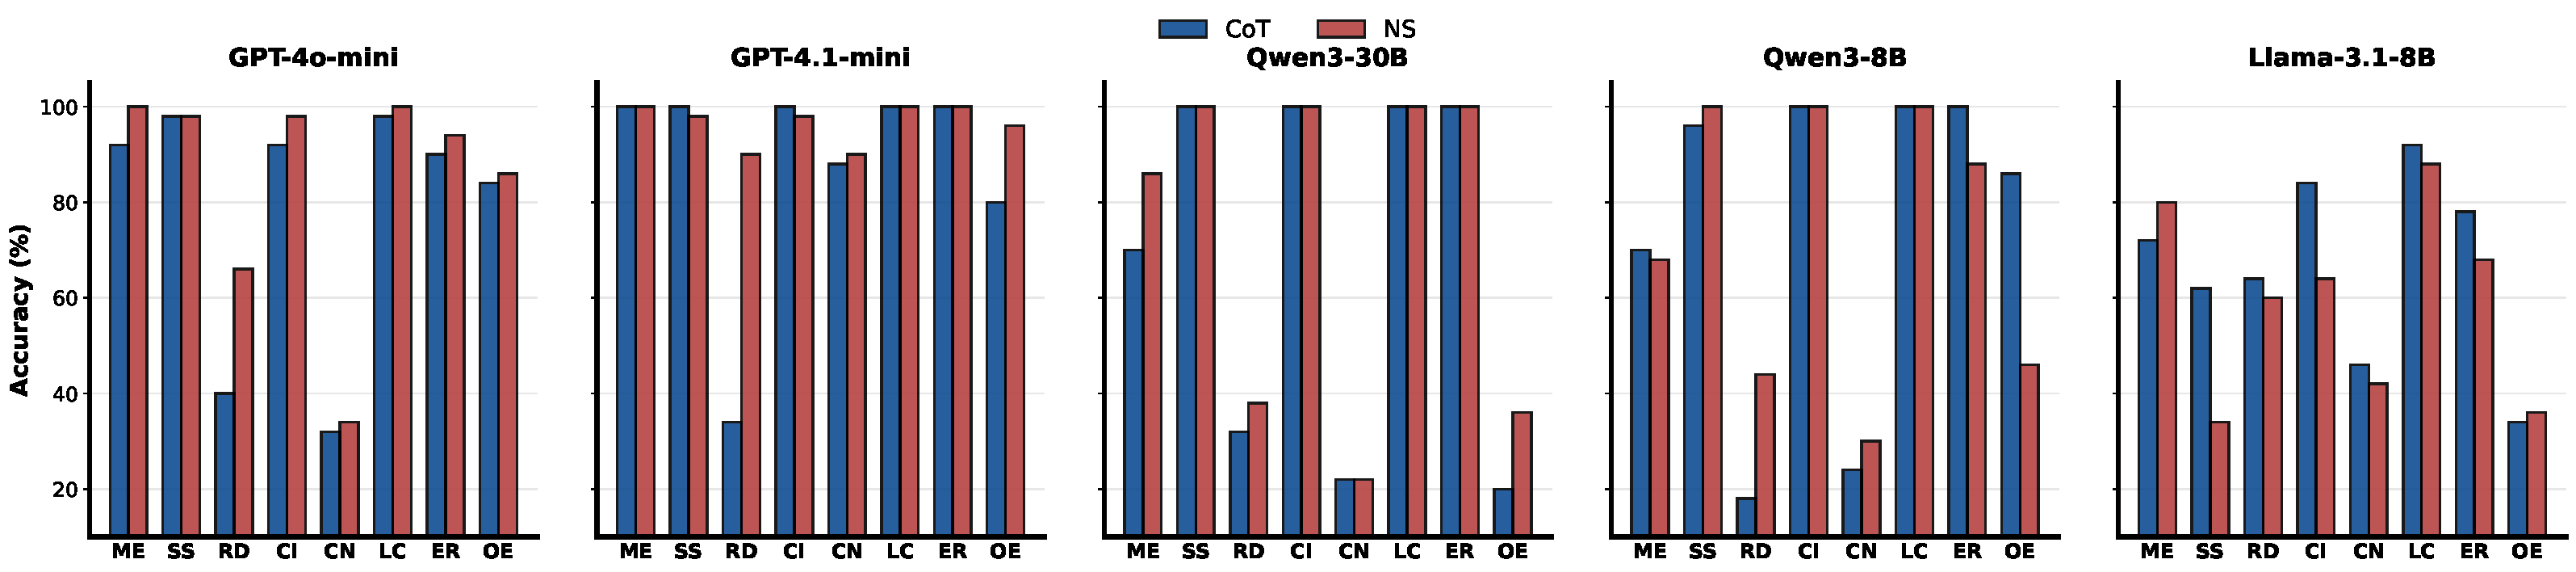
\includegraphics[width=\textwidth]{figures/fig_bar_d4.pdf}
    \caption{Per-category accuracy on strong-shortcut items at $d{=}4$. Blue = CoT, red = NS. Categories where NS exceeds CoT indicate effective shortcut activation; categories where NS falls below CoT indicate that estimation harms accuracy.}
    \label{fig:bar_d4}
\end{figure*}

The bar charts reveal qualitatively distinct profiles across models.
GPT-4o-mini and GPT-4.1-mini show NS improvements on most categories, with ME and LC reaching near-ceiling under NS.
Qwen3-30B and Qwen3-8B show NS benefits on ME and SS but drops on CN, LC, ER, and OE.
Llama-3.1-8B shows NS below CoT on most categories.

To account for differing CoT baselines across categories, Figure~\ref{fig:radar_norm} presents the normalized improvement $({\text{NS}} - {\text{CoT}}) / (1 - {\text{CoT}})$, measuring what fraction of the remaining accuracy gap NS captures.
GPT-4o-mini shows the broadest improvement profile, while Llama-3.1-8B is consistently negative.

\begin{figure}[t]
    \centering
    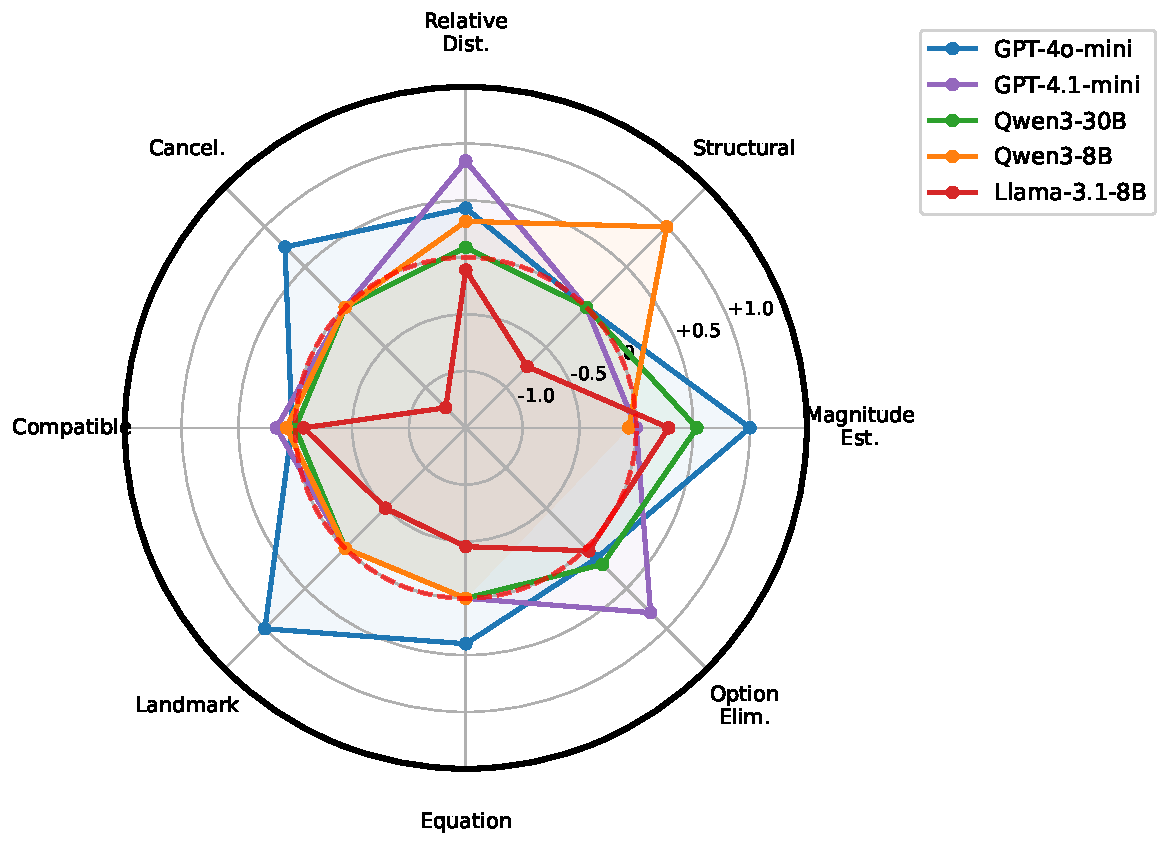
\includegraphics[width=0.7\textwidth]{figures/fig_radar_normalized_d4.pdf}
    \caption{Normalized NS improvement at $d{=}4$: $(\text{NS}-\text{CoT})/(1-\text{CoT})$. Values of $+1$ mean NS closes the entire remaining gap; $0$ means no change; negative means NS hurts. Red dashed line = zero.}
    \label{fig:radar_norm}
\end{figure}

These profiles suggest that number sense is not a single axis along which models can be ranked, but rather a multi-dimensional construct.
A model that excels at one shortcut type may perform at or below baseline on another.

\paragraph{Where NS hurts accuracy.}
NS reduces strong-item accuracy in several categories at $d{=}4$: option\_elimination ($-$44pp for Qwen3-8B), landmark\_comparison ($-$16pp), equation\_reasoning ($-$12pp), and magnitude\_estimation ($-$10pp).
These share a common trait: they require exact arithmetic or careful multi-step reasoning where estimation introduces fatal errors.
For equation reasoning, NS approximation compounds rounding errors (e.g., $3032+2697\approx5700$, but $5700-3391=2309$ instead of the exact 2338).
For option elimination with close distractors differing by 1--4 in the last digit, estimation cannot distinguish options.
By contrast, NS helps most on relative\_distance (+22pp for Qwen3-8B; +24pp for GPT-4o-mini), where CoT's extended reasoning introduces unnecessary computation.

Figures~\ref{fig:bar_d2}--\ref{fig:bar_d16} extend the per-category analysis to all digit scales, confirming that $d{=}4$ produces the most pronounced model-differentiated effects.

\begin{figure*}[t]
    \centering
    \begin{minipage}{0.49\textwidth}\centering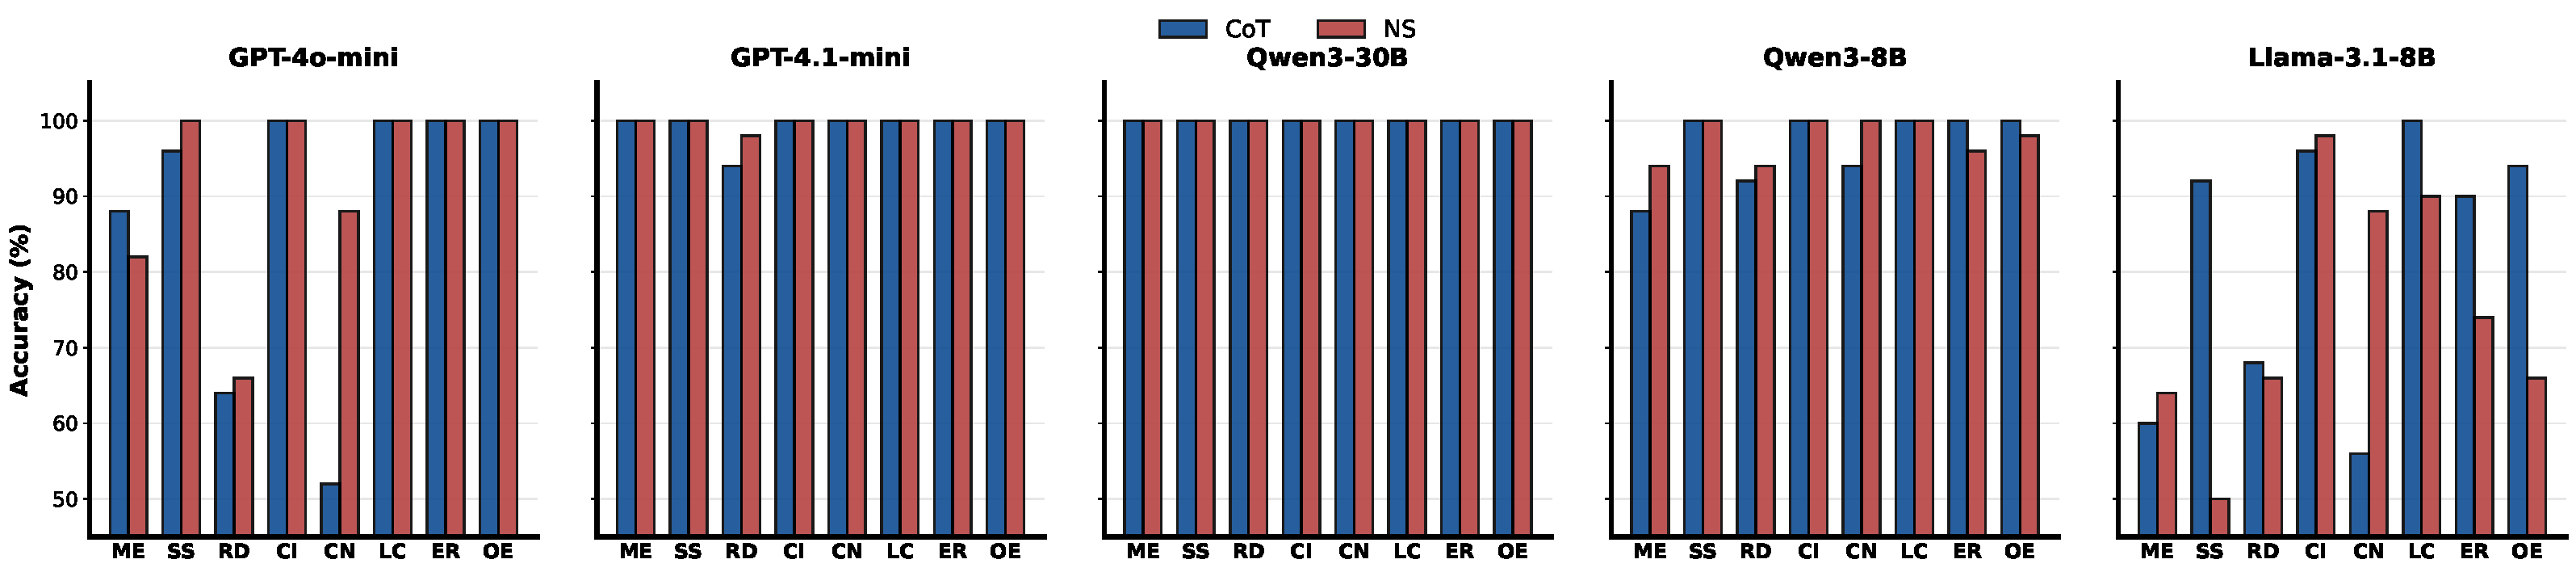
\includegraphics[width=\textwidth]{figures/fig_bar_d2.pdf}\caption{$d{=}2$}\label{fig:bar_d2}\end{minipage}
    \hfill
    \begin{minipage}{0.49\textwidth}\centering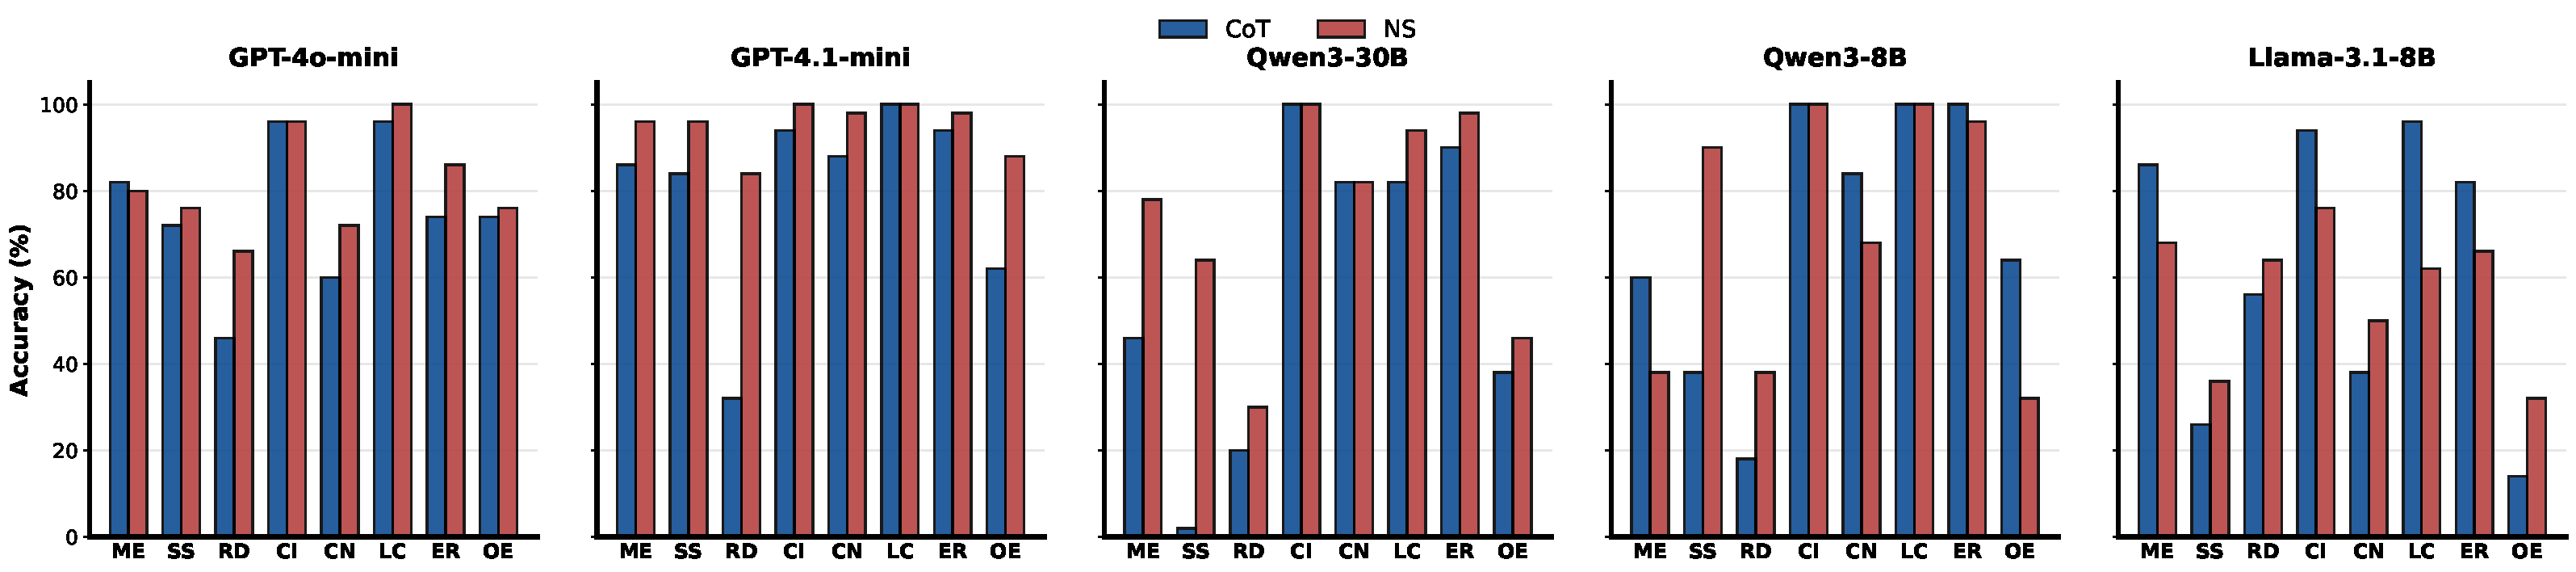
\includegraphics[width=\textwidth]{figures/fig_bar_d8.pdf}\caption{$d{=}8$}\label{fig:bar_d8}\end{minipage}
    \\[6pt]
    \begin{minipage}{0.49\textwidth}\centering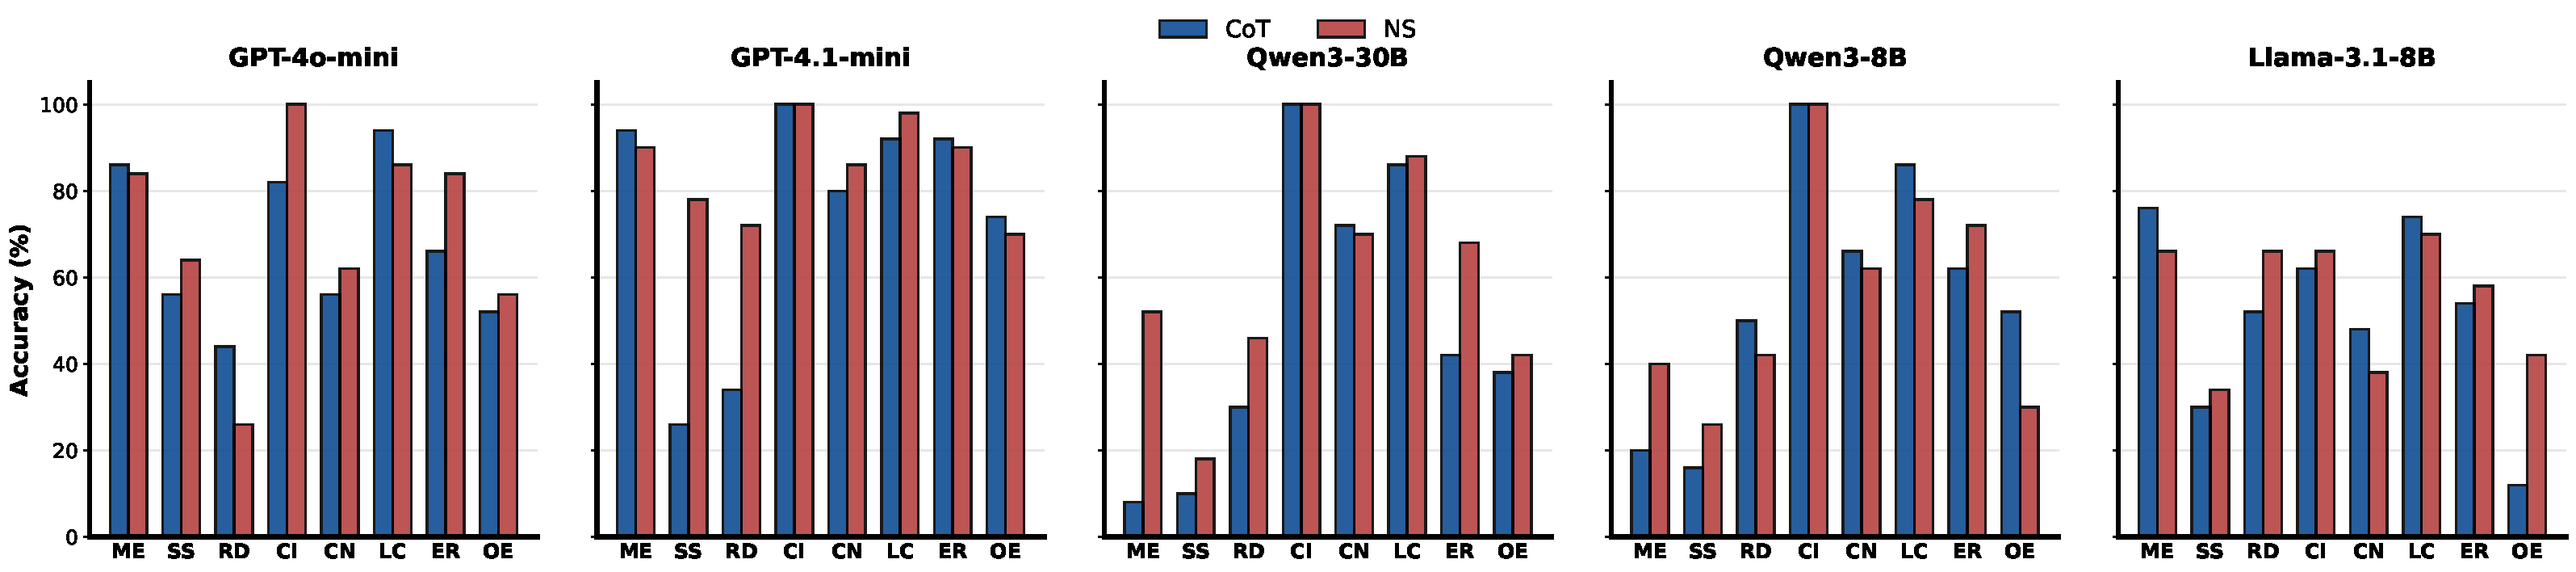
\includegraphics[width=\textwidth]{figures/fig_bar_d16.pdf}\caption{$d{=}16$}\label{fig:bar_d16}\end{minipage}
\end{figure*}

% ─────────────────────────────────────────────────────────────────────────────
\subsection{MATH-500 Number-Sense Analysis (Preliminary)}
\label{sec:math500}

As a preliminary test of whether number-sense prompting generalises beyond the controlled \textsc{SenseMath} items, we evaluate Qwen3-8B (base, no additional training) on MATH-500 \citep{hendrycks2021measuring}.

\paragraph{Annotation protocol.}
We partition MATH-500 into an \emph{NS-amenable} split and a \emph{computation-required} split using GPT-4.1-mini as a zero-shot classifier (temperature$\,{=}\,0$, $\texttt{max\_tokens}{=}10$).
Each problem is presented with the following prompt:
\begin{quote}
\small
\textit{You are classifying whether a math problem can benefit from Number Sense (NS) strategies (intuition, estimation, pattern recognition, magnitude reasoning, or structural shortcuts) or whether it fundamentally requires precise step-by-step algebraic/arithmetic computation. [\ldots] Reply with exactly one word: NS or COMP}
\end{quote}
This yields 171 NS-amenable problems (34.2\%) and 329 computation-required problems (65.8\%).
This classification task is structurally equivalent to our J1 judge task. The J1 accuracy across models (61--66\%) on the SenseMath dataset provides independent evidence that LLM-based classification of shortcut amenability is reliable.

\paragraph{Split results.}
On the NS-amenable split, Qwen3-8B under CoT achieves 84.8\% accuracy (avg.\ 262 tokens) versus NS at 83.0\% (avg.\ 235 tokens), a gap of only $\Delta = {-}1.8$pp with a 10.3\% token reduction.
On the computation-required split, CoT achieves 60.8\% (avg.\ 373 tokens) versus NS at 59.0\% (avg.\ 349 tokens), again $\Delta = {-}1.8$pp with a 6.4\% token reduction.

\paragraph{Key finding.}
Across both splits, the NS prompt causes minimal accuracy loss ($\leq 2$pp) on real MATH problems while consistently reducing token usage by 7--10\%.
This supports the practical viability of number-sense prompting as a drop-in efficiency improvement for math-capable models.

% ─────────────────────────────────────────────────────────────────────────────
\subsection{Strict Prompt Validation}
\label{sec:strict}

The Strict condition provides a negative control: by explicitly forbidding shortcuts, it should suppress shortcut-based reasoning and lower accuracy on strong-shortcut items.
We report Strict results for GPT-4o-mini only, because the open-weight models (Qwen, Llama) frequently truncate their Strict responses at the 512-token limit, rendering accuracy estimates unreliable.

\paragraph{GPT-4o-mini Strict results.}
At $d{=}4$, the gap between NS and Strict is substantial: NS achieves 84.5\% on strong items versus Strict's 90.5\%, but Strict control accuracy (87.2\%) far exceeds NS control accuracy (63.0\%).
Qualitative analysis of keyword frequencies in GPT-4o-mini outputs supports the interpretation: Strict responses contain shortcut-related keywords (e.g., ``approximately'', ``round'', ``cancel'') in only 11\% of responses, compared to 46\% under CoT and 87\% under NS.
This gradient, Strict $<$ CoT $<$ NS, is consistent with the view that CoT partially activates shortcuts (see \S\ref{sec:cot_strategy}), while NS maximally activates them and Strict effectively suppresses them.

\paragraph{Truncation caveat.}
For the three open-weight models, Strict prompting produces responses that exceed 512 tokens on 30--60\% of items (the instruction to show all arithmetic steps inflates response length).
Because truncated responses lack a \boxed{} answer and are scored as incorrect, accuracy under Strict is systematically deflated for these models.
We therefore treat Strict as a validation condition rather than a primary comparison, and restrict Strict-based analyses to GPT-4o-mini.

% ─────────────────────────────────────────────────────────────────────────────
\subsection{CoT Strategy Analysis}
\label{sec:cot_strategy}

An important nuance is that CoT does not uniformly produce pure computation.
Qualitative inspection of CoT responses reveals that models sometimes discover and apply shortcuts even without explicit prompting, particularly on strong-shortcut items with salient numerical structure.

For example, on a cancellation item ($3{,}456 + 7{,}891 - 7{,}889$), GPT-4o-mini's CoT response begins with standard addition but then states ``I notice $7{,}891 - 7{,}889 = 2$'' and immediately produces the correct answer.
Similarly, Qwen3-30B's CoT responses on structural-shortcut items frequently invoke the distributive law (``$99 \times 37 = (100-1) \times 37$'') without being prompted to look for such decompositions.

This spontaneous shortcut discovery under CoT has two implications.
First, it suggests that some degree of number-sense reasoning is embedded in these models' default behaviour and does not require explicit elicitation.
Second, and more importantly for interpreting our results, it means that the NS--CoT comparison is \emph{conservative}: the NS condition activates shortcuts that CoT does not, but CoT already activates some shortcuts on its own.
The NS--Strict comparison, where Strict suppresses even spontaneous shortcuts, produces a wider gap.

This conservatism strengthens the interpretation: even against a partially shortcut-aware CoT baseline, the NS prompt produces a measurable additional asymmetric effect on shortcut-amenable items.

\paragraph{Strategy-use quantification.}
To move beyond accuracy and directly measure strategy choice, we use GPT-4.1-mini as a judge to classify every model response as SHORTCUT or COMPUTATION across all five models and all digit scales.
The NS\% rows in Table~\ref{tab:main_results} report the results.
Under CoT, shortcut rates are low (20--39\% at $d{=}4$) with a consistent strong$>$control gap for Qwen3-30B and Qwen3-8B, confirming that shortcut-amenable items spontaneously elicit more shortcut reasoning.
NS prompting dramatically increases shortcut use to 68--86\% across all models, scales, and variants.
Crucially, the NS shortcut rate is similar on strong and control items (e.g., Qwen3-8B at $d{=}4$: 86\% strong, 88\% control).
This reveals the mechanism behind the accuracy asymmetry: NS induces shortcut strategies uniformly, but these strategies succeed on strong items (where valid shortcuts exist) and fail on control items (where no shortcut applies).

% ─────────────────────────────────────────────────────────────────────────────
\subsection{Judge and Generate Tasks}
\label{sec:judge_generate}

We evaluate declarative shortcut knowledge through Judge tasks and constructive shortcut ability through Generate tasks.

\paragraph{J1: Shortcut appropriateness.}
Models are asked whether a number-sense shortcut would be effective for a given problem (YES/NO), evaluated on 251 items after filtering.
GPT-4o-mini achieves the highest J1 accuracy (66.3\%), with perfect recognition of shortcut-amenable items (100\% on strong) but complete failure to reject non-shortcut items (0\% on control). It says YES to every item.
GPT-4.1-mini scores 65.3\% overall with a more balanced profile (89.1\% strong, 15.8\% control), suggesting better calibration at the cost of lower shortcut recognition.
Qwen3-8B follows at 65.0\% (97.8\% strong, 0\% control), exhibiting the same extreme YES bias as GPT-4o-mini.
Qwen3-30B scores 64.0\% (96.7\% strong, 4.0\% control), also strongly biased toward YES.
Llama-3.1-8B scores 61.3\% (82.6\% strong, 20.8\% control), showing a relatively more balanced profile among the tested models.
The near-zero control accuracy for most models reflects over-rationalization: given any problem, the model can construct a plausible shortcut strategy, making it unable to reject control items.

\paragraph{J2: Strategy identification.}
Given a problem and its solution, models classify whether the solution used a shortcut or computation strategy (SHORTCUT/COMPUTATION).
The J2 dataset comprises 80 verified items: 54 SHORTCUT cases drawn from NS responses on strong-shortcut items, and 26 COMPUTATION cases drawn from CoT responses on control items; all labels were confirmed by manual audit.
GPT-4.1-mini achieves the highest J2 accuracy (91.2\%), with balanced performance on both SHORTCUT (90.7\%) and COMPUTATION (92.3\%) identification.
GPT-4o-mini correctly identifies shortcuts in 94.0\% of cases but misclassifies computation as shortcut in 42\% of cases, suggesting a liberal bias toward labelling solutions as shortcut-based.

\paragraph{G2: Problem generation.}
Models generate novel shortcut/control problem pairs from a category description and one example, verified by 6 deterministic code checks.
Qwen3-30B leads at 25\% pass rate, followed by Qwen3-8B (20\%), GPT-4.1-mini (18\%), GPT-4o-mini (9\%), and Llama-3.1-8B (2\%). All models are evaluated on 96 prompts (8 categories $\times$ 12).
The primary bottleneck is constructing expressions where a valid shortcut exists: the shortcut-existence check fails on 51\% of generated items across all models.
A common failure mode is generating numerically plausible strong items where the intended structure (e.g., operand near a power of 10) is too weak to qualify as a genuine shortcut.

Table~\ref{tab:judge} and Table~\ref{tab:generate} present the full results.

\begin{table}[t]
\centering
\small
\caption{Judge task results. J1: shortcut appropriateness (251 items). J2: strategy identification (80 items). \textcolor{green!60!black}{Green}/\textcolor{red!70!black}{red} = gap from ideal (100\% for strong, 100\% for control).}
\label{tab:judge}
\begin{tabular}{llrrr}
\toprule
Task & Model & Overall (\%) & Strong (\%) & Control (\%) \\
\midrule
J1 & GPT-4o-mini  & 66 & 100 & 0 \textcolor{red!70!black}{\scriptsize $-$100} \\
   & GPT-4.1-mini & 65 & 89 \textcolor{red!70!black}{\scriptsize $-$11} & 16 \textcolor{red!70!black}{\scriptsize $-$84} \\
   & Qwen3-8B     & 65 & 98 \textcolor{red!70!black}{\scriptsize $-$2} & 0 \textcolor{red!70!black}{\scriptsize $-$100} \\
   & Qwen3-30B    & 64 & 97 \textcolor{red!70!black}{\scriptsize $-$3} & 4 \textcolor{red!70!black}{\scriptsize $-$96} \\
   & Llama-3.1-8B & 61 & 83 \textcolor{red!70!black}{\scriptsize $-$17} & 21 \textcolor{red!70!black}{\scriptsize $-$79} \\
\midrule
 & & Overall (\%) & SHORTCUT (\%) & COMP (\%) \\
\midrule
J2 & GPT-4.1-mini & 91 & 91 & 92 \\
   & GPT-4o-mini  & 70 \textcolor{red!70!black}{\scriptsize $-$21} & 94 \textcolor{green!60!black}{\scriptsize +3} & 58 \textcolor{red!70!black}{\scriptsize $-$34} \\
\bottomrule
\end{tabular}
\end{table}

\begin{table}[t]
\centering
\small
\caption{G2 problem generation: per-check pass rates (\%) and 6/6 pass. All models evaluated on 96 prompts (8 categories $\times$ 12). \textcolor{green!60!black}{Green}/\textcolor{red!70!black}{red} = delta from top model per column.}
\label{tab:generate}
\setlength{\tabcolsep}{3pt}
\begin{tabular}{l r rrrrrr r}
\toprule
Model & Fmt & S.Ans & C.Ans & SC.Ex & C.Blk & Fam & Nov & Pass \\
\midrule
Qwen3-30B    & 96 & 65 & 73 & 66 & 87 & 76 & 96 & 23/96 \\
Qwen3-8B     & 100 & 69 \textcolor{green!60!black}{\scriptsize+4} & 64 \textcolor{red!70!black}{\scriptsize$-$9} & 55 \textcolor{red!70!black}{\scriptsize$-$11} & 83 \textcolor{red!70!black}{\scriptsize$-$4} & 71 \textcolor{red!70!black}{\scriptsize$-$5} & 99 \textcolor{green!60!black}{\scriptsize+3} & 19/96 \\
GPT-4.1-mini & 100 & 70 \textcolor{green!60!black}{\scriptsize+5} & 79 \textcolor{green!60!black}{\scriptsize+6} & 67 \textcolor{green!60!black}{\scriptsize+1} & 80 \textcolor{red!70!black}{\scriptsize$-$7} & 75 \textcolor{red!70!black}{\scriptsize$-$1} & 94 \textcolor{red!70!black}{\scriptsize$-$2} & 17/96 \\
GPT-4o-mini  & 100 & 58 \textcolor{red!70!black}{\scriptsize$-$7} & 48 \textcolor{red!70!black}{\scriptsize$-$25} & 46 \textcolor{red!70!black}{\scriptsize$-$20} & 82 \textcolor{red!70!black}{\scriptsize$-$5} & 73 \textcolor{red!70!black}{\scriptsize$-$3} & 88 \textcolor{red!70!black}{\scriptsize$-$8} & 9/96 \\
Llama-3.1-8B & 100 & 51 \textcolor{red!70!black}{\scriptsize$-$14} & 46 \textcolor{red!70!black}{\scriptsize$-$27} & 38 \textcolor{red!70!black}{\scriptsize$-$28} & 83 \textcolor{red!70!black}{\scriptsize$-$4} & 52 \textcolor{red!70!black}{\scriptsize$-$24} & 90 \textcolor{red!70!black}{\scriptsize$-$6} & 2/96 \\
\bottomrule
\end{tabular}
\end{table}


\begin{figure}[t]
\centering
\small
\fbox{\parbox{0.93\columnwidth}{%
\textbf{G2 Pass} (Qwen3-30B, magnitude\_estimation).\\
Strong: $10{,}200 \times 9{,}800 = 99{,}960{,}000$ \checkmark\quad
Control: $4{,}321 \times 5{,}678 = 24{,}537{,}538$ \checkmark\\
Both operands near $10^4$ in strong $\Rightarrow$ shortcut exists; control operands far from round numbers $\Rightarrow$ shortcut blocked. All 6 checks pass.\\[6pt]
%
\textbf{G2 Fail} (Qwen3-30B, magnitude\_estimation).\\
Strong: $10{,}200 \times 9{,}850$; model claims $= 100{,}000{,}000$, actual $= 100{,}470{,}000$ \ding{55}\\
The model rounded too aggressively ($10{,}200 \approx 10{,}000$, $9{,}850 \approx 10{,}000$) and reported the estimate as the exact answer. The shortcut-existence check passes, but the answer-correctness check fails.
}}
\caption{G2 generation examples. Pass: model produces a valid shortcut/control pair. Fail: model confuses its own shortcut estimate with the exact answer.}
\label{fig:g2_case}
\end{figure}

% ─────────────────────────────────────────────────────────────────────────────
\subsection{Post-Training (Preliminary): Can Number Sense Be Trained?}
\label{sec:training}

The prompting experiments establish that number-sense shortcuts can be elicited at inference time.
A natural follow-up asks whether targeted \emph{training} can internalize number-sense reasoning more durably.
We present a proof-of-concept study using Qwen3-8B fine-tuned with Direct Preference Optimization (DPO) on 500 MATH problems, pairing NS-style shortcut solutions (generated by GPT-5.1) as preferred responses against verbose CoT solutions as rejected responses.
Training uses LoRA (rank 8, all linear layers) with LLaMA-Factory; full hyperparameters appear in the supplementary material.

\paragraph{Combined-DPO results.}
After training, Qwen3-8B achieves 68.0\% accuracy under NS prompting on a held-out 200-problem MATH evaluation set, an improvement of ${+}3.0$pp over the base model (65.0\%).
Average token usage increases modestly to 375 tokens from 340 in the base model, reflecting slightly longer shortcut explanations in the fine-tuned outputs.

\paragraph{Out-of-distribution (OOD) generalization.}
To verify that training on number-sense examples does not harm general capabilities, we evaluate the fine-tuned model on 7 standard benchmarks.
All results fall within $\pm 4$pp of the base model: BBH 73.8\%$\to$69.8\%, ARC 87.0\%$\to$87.0\%, and similar small changes across the remaining five benchmarks.
Table~\ref{tab:ood} presents the full OOD comparison.

\begin{table}[t]
\centering
\caption{Out-of-distribution benchmark results after 500-example training. Most variants fall within $\pm$4pp of base, confirming no catastrophic forgetting.}
\label{tab:ood}
\small
\setlength{\tabcolsep}{3.5pt}
\begin{tabular}{ll ccccccc}
\toprule
Model & Variant & BBH & ARC & GPQA & MMLU-P & MedQA & LogiQA & CSQA \\
\midrule
Qwen3-8B & Base         & 73.8 & 87.0 & 34.6 & 31.8 & 61.4 & 50.5 & 80.8 \\
         & NS-DPO       & 73.8 & 87.0 & 31.2 & 31.4 & 59.4 & 46.9 & 80.8 \\
         & Baseline-DPO & 73.6 & 86.6 & 34.6 & 31.8 & 59.0 & 47.9 & 80.7 \\
         & NS-SFT       & 73.6 & 86.6 & 33.7 & 32.6 & 60.4 & 48.4 & 80.7 \\
         & CoT-SFT      & 73.4 & 86.3 & 32.8 & 30.6 & 60.6 & 48.7 & 80.9 \\
         & Comb-SFT     & --- & --- & --- & --- & --- & --- & --- \\
         & Comb-DPO     & 69.8 & 87.0 & 35.0 & 28.4 & 62.2 & 51.0 & 80.0 \\
\midrule
Llama-3-8B & Base       & 50.2 & 80.3 & 29.2 & 19.2 & 60.6 & 41.6 & 75.4 \\
           & NS-DPO     & 49.8 & 80.6 & 28.6 & 19.4 & 59.6 & 42.4 & 75.7 \\
           & Baseline-DPO & 50.2 & 80.3 & 28.8 & 18.4 & 60.2 & 42.1 & 75.7 \\
           & NS-SFT     & 50.6 & 80.3 & 28.8 & 18.8 & 60.4 & 42.4 & 75.8 \\
           & CoT-SFT    & 50.4 & 80.3 & 29.9 & 19.0 & 60.4 & 41.8 & 75.9 \\
           & Comb-SFT   & 54.4 & 82.6 & 27.9 & 17.4 & 59.4 & 40.9 & 74.6 \\
           & Comb-DPO   & 54.4 & 82.3 & 29.2 & 18.0 & 59.6 & 41.0 & 74.5 \\
\bottomrule
\end{tabular}
\end{table}


\begin{table}[t]
\centering
\caption{In-domain results on the 200-problem eval set (500-example training). NS Rate = fraction of responses using number-sense strategy; Avg Tok = average response tokens. Best accuracy per model per prompt condition is \textbf{bold}.}
\label{tab:training}
\small
\begin{tabular}{ll l ccc}
\toprule
Model & Variant & Prompt & NS Rate & Accuracy & Avg Tok \\
\midrule
Qwen3-8B   & Base          & CoT & 10.0\% & 64.5\%          & 376 \\
(nothink)  & Base          & NC  & 36.5\% & 65.0\%          & 340 \\
           & NS-DPO        & CoT & 11.5\% & \textbf{67.0\%} & 372 \\
           & NS-DPO        & NC  & 33.5\% & 64.0\%          & 350 \\
           & Baseline-DPO  & CoT &  8.5\% & 66.0\%          & 374 \\
           & Baseline-DPO  & NC  & 34.5\% & 60.0\%          & 350 \\
           & NS-SFT        & CoT & 11.5\% & 66.0\%          & 369 \\
           & NS-SFT        & NC  & 32.5\% & 64.0\%          & 348 \\
           & CoT-SFT       & CoT & 11.5\% & 64.0\%          & 373 \\
           & CoT-SFT       & NC  & 34.5\% & 63.0\%          & 351 \\
           & Combined-SFT  & CoT & 11.5\% & 63.0\%          & 392 \\
           & Combined-SFT  & NC  & 22.0\% & 65.5\%          & 372 \\
           & Combined-DPO  & CoT & 11.0\% & 62.5\%          & 395 \\
           & Combined-DPO  & NC  & 23.5\% & \textbf{68.0\%} & 375 \\
\midrule
Llama-3-8B & Base          & CoT &  5.5\% & 21.5\%          & 363 \\
           & Base          & NC  & 44.5\% & 15.5\%          & 269 \\
           & NS-DPO        & CoT &  3.5\% & 22.5\%          & --- \\
           & NS-DPO        & NC  & 48.0\% & 17.0\%          & --- \\
           & Baseline-DPO  & CoT &  4.5\% & 18.5\%          & --- \\
           & Baseline-DPO  & NC  & 51.0\% & 17.0\%          & --- \\
           & NS-SFT        & CoT &  3.5\% & 24.0\%          & 398 \\
           & NS-SFT        & NC  & 57.5\% & 16.0\%          & 285 \\
           & CoT-SFT       & CoT &  3.0\% & 25.0\%          & 379 \\
           & CoT-SFT       & NC  & 59.0\% & 19.0\%          & 292 \\
           & Combined-SFT  & CoT &  4.0\% & \textbf{37.5\%} & 321 \\
           & Combined-SFT  & NC  & 16.0\% & 31.5\%          & 286 \\
           & Combined-DPO  & CoT &  4.5\% & 36.5\%          & 325 \\
           & Combined-DPO  & NC  & 12.0\% & 30.0\%          & 288 \\
\bottomrule
\end{tabular}
\end{table}


\paragraph{Conclusion.}
Small-scale DPO training (500 examples) on number-sense-preferred solutions improves shortcut exploitation by up to 3pp without degrading generalization across seven diverse OOD benchmarks (Table~\ref{tab:ood}).
This demonstrates that number sense is a trainable capability, and that the prompt-level effects observed in the main experiments can be amplified through targeted post-training.

\section{Conclusion}
\label{sec:conclusion}

This work introduced \textsc{SenseMath}, a controlled benchmark that measures prompt-sensitive shortcut exploitation on matched item families.
By pairing strong-shortcut, weak-shortcut, and control variants within each family, the benchmark isolates the prompting asymmetry from confounds such as general prompt quality or item difficulty.

Our experiments across five models yield three main findings.
First, a category-agnostic NS prompt produces an asymmetric effect at $d{=}4$: accuracy on shortcut-amenable items is maintained or improved while accuracy on matched controls drops, most consistently for GPT-4o-mini and Qwen3-8B.
Second, per-category radar profiles reveal that models show selective strengths and reversals across shortcut types. Qwen models lead on magnitude estimation and structural shortcuts, while GPT-4o-mini dominates cancellation, equation reasoning, and option elimination. This establishes number sense as a multi-dimensional construct rather than a single ability.
Third, a three-level evaluation (Use, Judge, Generate) reveals crossed dissociations: models that exploit shortcuts well do not necessarily recognise when shortcuts apply, and vice versa.

\paragraph{Limitations.}
Several limitations qualify these findings.
We have not conducted a human behavioural study to anchor LLM performance against human number sense; such a study is planned but not yet complete.
The benchmark contains 50 families per category, which is sufficient for detecting moderate-to-large effects but limits statistical power for fine-grained within-category analyses.
The Strict prompting condition produces truncated responses for open-weight models at 512 tokens, restricting its use as a negative control to GPT-4o-mini.
The multiple-choice format constrains the space of possible responses; free-response evaluation would provide richer signal about the reasoning process.
Finally, the 8 categories, while grounded in the mathematics education literature, are not exhaustive. Other shortcut types (e.g., modular arithmetic, dimensional analysis) remain untested.

\paragraph{Future directions.}
Several extensions follow naturally from this work.
A human validation study would establish whether the shortcut profiles we observe in LLMs mirror human number-sense behaviour.
Moving from multiple-choice to free-response items would allow finer-grained analysis of how models construct shortcut strategies.
Evaluating additional models, particularly reasoning-specialised systems and larger open-weight models, would clarify how number sense scales with model capability and training data.
Finally, the asymmetric prompting effects documented here suggest that shortcut-sensitive reasoning is in principle trainable; targeted fine-tuning on curated shortcut solutions could shift models from algorithmic defaults toward more flexible numerical reasoning.


\bibliography{references}
\bibliographystyle{colm2026_conference}

\appendix

\section{Example Items}
\label{sec:appendix_examples}

Table~\ref{tab:examples} shows example \textsc{SenseMath} items at $d{=}2$ for four categories.

\begin{table*}[t]
\centering
\small
\caption{Example \textsc{SenseMath} items ($d{=}2$). Each row shows one family; the strong variant admits a clean shortcut while the control requires direct computation. Correct answers are \textbf{bolded}.}
\label{tab:examples}
\begin{tabular}{@{}p{1.5cm}p{5.7cm}p{5.7cm}@{}}
\toprule
\textbf{Category} & \textbf{Strong-shortcut variant} & \textbf{Control variant} \\
\midrule
Structural (SS) &
\emph{What is $98 \times 34$?} \newline
(A)~3322 \quad (B)~3342 \quad \textbf{(C)~3332} \quad (D)~3352 \newline
{\footnotesize Shortcut: $98{=}(100{-}2)$, so $100{\times}34 - 2{\times}34 = 3332$.} &
\emph{What is $47 \times 40$?} \newline
(A)~1870 \quad (B)~1890 \quad (C)~1900 \quad \textbf{(D)~1880} \newline
{\footnotesize No near-100 structure; direct multiplication required.} \\
\addlinespace
Cancellation (CI) &
\emph{Evaluate: $71 + 28 - 27$.} \newline
(A)~82 \quad (B)~92 \quad \textbf{(C)~72} \quad (D)~62 \newline
{\footnotesize Shortcut: $28{-}27{=}1$, so $\approx 71{+}1 = 72$.} &
\emph{Evaluate: $71 + 28 - 118$.} \newline
(A)~$-19$ \quad (B)~$-1$ \quad \textbf{(C)~$-11$} \quad (D)~$-31$ \newline
{\footnotesize No near-cancellation; full arithmetic needed.} \\
\addlinespace
Equation (ER) &
\emph{$23 + 22 = \rule{0.5cm}{0.4pt} + 18$.} \newline
(A)~37 \quad \textbf{(B)~27} \quad (C)~47 \quad (D)~17 \newline
{\footnotesize Shortcut: move 18 left, $23{+}22{-}18 = 27$.} &
\emph{$20 + 93 + \rule{0.5cm}{0.4pt} = 59 + 49$.} \newline
(A)~15 \quad (B)~$-15$ \quad \textbf{(C)~$-5$} \quad (D)~5 \newline
{\footnotesize No direct identity; must compute both sides.} \\
\addlinespace
Option Elim (OE) &
\emph{What is $70 \times 16$?} \newline
(A)~1123 \quad (B)~1119 \quad (C)~1121 \quad \textbf{(D)~1120} \newline
{\footnotesize Shortcut: $70{\times}\text{even} \Rightarrow$ ends in 0; only 1120 qualifies.} &
\emph{What is $33 \times 87$?} \newline
(A)~3031 \quad (B)~2973 \quad (C)~3187 \quad \textbf{(D)~2871} \newline
{\footnotesize All options plausible; no elimination possible.} \\
\bottomrule
\end{tabular}
\end{table*}


\section{Prompt Templates}
\label{sec:appendix_prompts}

\textbf{CoT:} ``Please solve the following multiple-choice problem. Show your step-by-step reasoning, then provide your final answer as a single capital letter (A, B, C, or D) inside \textbackslash boxed\{\}.''

\textbf{NS:} ``Please solve the following multiple-choice problem using only easy calculations. Rely on your mathematical intuition, number sense, and estimation. Show brief reasoning, then provide your final answer as a single capital letter (A, B, C, or D) inside \textbackslash boxed\{\}.''

\textbf{Strict:} ``Please solve the following multiple-choice problem by performing precise, step-by-step arithmetic. Do NOT use estimation, rounding, or shortcuts. Show every computation digit by digit, then provide your final answer as a single capital letter (A, B, C, or D) inside \textbackslash boxed\{\}.''

\section{Task Specifications}
\label{sec:appendix_tasks}

\paragraph{J1 prompt:} ``Consider this math problem. Could you solve it significantly faster using mental math or a clever observation, compared to computing it step by step? Answer YES or NO, then explain in one sentence why.''

\paragraph{J2 prompt:} ``Classify the solution strategy as SHORTCUT or COMPUTATION. SHORTCUT: uses estimation, approximation, pattern recognition, structural insight, cancellation, or benchmark comparison. COMPUTATION: performs standard step-by-step arithmetic.''

\paragraph{G2:} Models receive a category description and one example strong/control pair, then generate a new pair in JSON format. Six deterministic code checks verify: (1) strong answer correctness, (2) control answer correctness, (3) shortcut existence in strong, (4) shortcut absence in control, (5) family matching, (6) novelty and digit scale.

\paragraph{Heuristic validation.} A deterministic shortcut solver applies category-specific heuristics without exact arithmetic. On strong items it achieves $\geq 70\%$; on control items approximately 25\%, confirming a 40pp separation.

\paragraph{Benchmark integrity.} All distractors share the last 50\% of digits (arithmetic) or fall within $\pm 0.1$ decimal (fractions). Correct option position is balanced across A/B/C/D.

\section{Strict Condition Results}
\label{sec:appendix_strict}

Table~\ref{tab:strict} presents Strict accuracy at $d{=}4$. High truncation for open-weight models (76--97\%) deflates their estimates.

\begin{table*}[t]
\centering
\small
\caption{Strict condition results (\%) across all digit scales. Strict instructs digit-by-digit computation without shortcuts. Open-weight models truncate at 512 tokens; GPT models at 1024. $S$ = strong, $W$ = weak, $C$ = control. NS\% confirms Strict effectively suppresses shortcut strategies (0--9\% at $d{=}4$).}
\label{tab:strict}
\begin{tabular}{ll|rrr|rrr|rrr|rrr}
\toprule
 & & \multicolumn{3}{c|}{$d=2$} & \multicolumn{3}{c|}{$d=4$} & \multicolumn{3}{c|}{$d=8$} & \multicolumn{3}{c}{$d=16$} \\
Model & Metric & $S$ & $W$ & $C$ & $S$ & $W$ & $C$ & $S$ & $W$ & $C$ & $S$ & $W$ & $C$ \\
\midrule
GPT-4o-mini  & Acc  & 94 & 96 & 92 & 83 & 78 & 83 & 70 & 58 & 48 & 68 & 58 & 45 \\
             & NS\% & 2 & 2 & 1 & 3 & 0 & 0 & 8 & 0 & 0 & 12 & 2 & 0 \\
\midrule
GPT-4.1-mini & Acc  & 100 & 99 & 100 & 91 & 90 & 90 & 60 & 54 & 29 & 55 & 35 & 36 \\
             & NS\% & 6 & 0 & 0 & 9 & 0 & 0 & 18 & 1 & 0 & 26 & 13 & 26 \\
\midrule
Qwen3-30B    & Acc  & 89 & 89 & 92 & 26 & 25 & 20 & 24 & 24 & 24 & 34 & 28 & 34 \\
             & NS\% & 0 & 0 & 0 & 2 & 0 & 0 & 11 & 4 & 0 & 20 & 10 & 5 \\
\midrule
Qwen3-8B     & Acc  & 91 & 92 & 92 & 53 & 46 & 44 & 37 & 34 & 41 & 33 & 28 & 26 \\
             & NS\% & 1 & 0 & 0 & 6 & 0 & 1 & 8 & 0 & 0 & 20 & 4 & 6 \\
\midrule
Llama-3.1-8B & Acc  & 55 & 62 & 61 & 46 & 50 & 40 & 36 & 36 & 30 & 22 & 23 & 20 \\
             & NS\% & 0 & 0 & 0 & 0 & 0 & 0 & 1 & 0 & 0 & 4 & 0 & 0 \\
\bottomrule
\end{tabular}
\end{table*}


\end{document}
